\chapter{Planning and Budget}
\label{ch:planning-and-budget}

\section{Planning}
The planning of this work covers from the moment the proposal for the teaching commission began
to be made until the moment the work is presented publicly. Of course there are some milestones
that are fixed in time such as \textbf{the presentation of the proposal}, \textbf{the presentation of the dissertation}
and \textbf{the defense of the work}. Therefore planning revolves around these milestones \textit{(IDs
3, 4 and 5 from \cref{fig:planning-sheet})}.

\subsection{Presentation of the Proposal}
The acceptance of the proposal includes the first tasks \textit{(IDs
6-8 from \cref{fig:planning-sheet})} in which a small investigation is done on the
topics of interest and it is decided what the objectives to be pursued of the work will be.

In addition, it also includes the formal preparation of the proposal that will be delivered to the
management of the computer engineering school for evaluation.

\subsection{Presentation of the Dissertation}
To consider the presentation of the dissertation as complete, it is necessary to carry out the main
tasks \textit{(IDs 9-34 from \cref{fig:planning-sheet})} of the work, in our case they are to
carry out the corresponding research to understand the scope of the proposed objectives, to propose a
solution and to obtain a few relustados that can be empirically testable. So that we can evaluate our
solutions. And, of course, prepare the corresponding documentation that reflects all the work done.

\subsection{Defense of the Work}
The defense of the project corresponds to those tasks \textit{(IDs 34-36 from \cref{fig:planning-sheet})}
subsequent to the delivery of the dissertation and that have to do with public defense in which the work carried out is evaluated.

\bigskip
So as you can see the main project statistics are shown in \cref{tb:planning-stats}.

\begin{table}
    \caption[Statistics of the main project tasks]{Statistics of the main project tasks.}
    \label{tb:planning-stats}
    \centering
    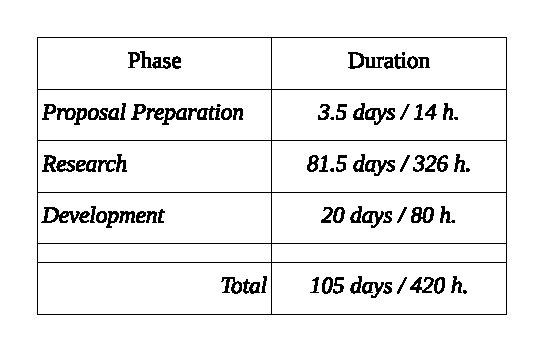
\includegraphics{images/planning-stats.pdf}
\end{table}

\begin{figure}
    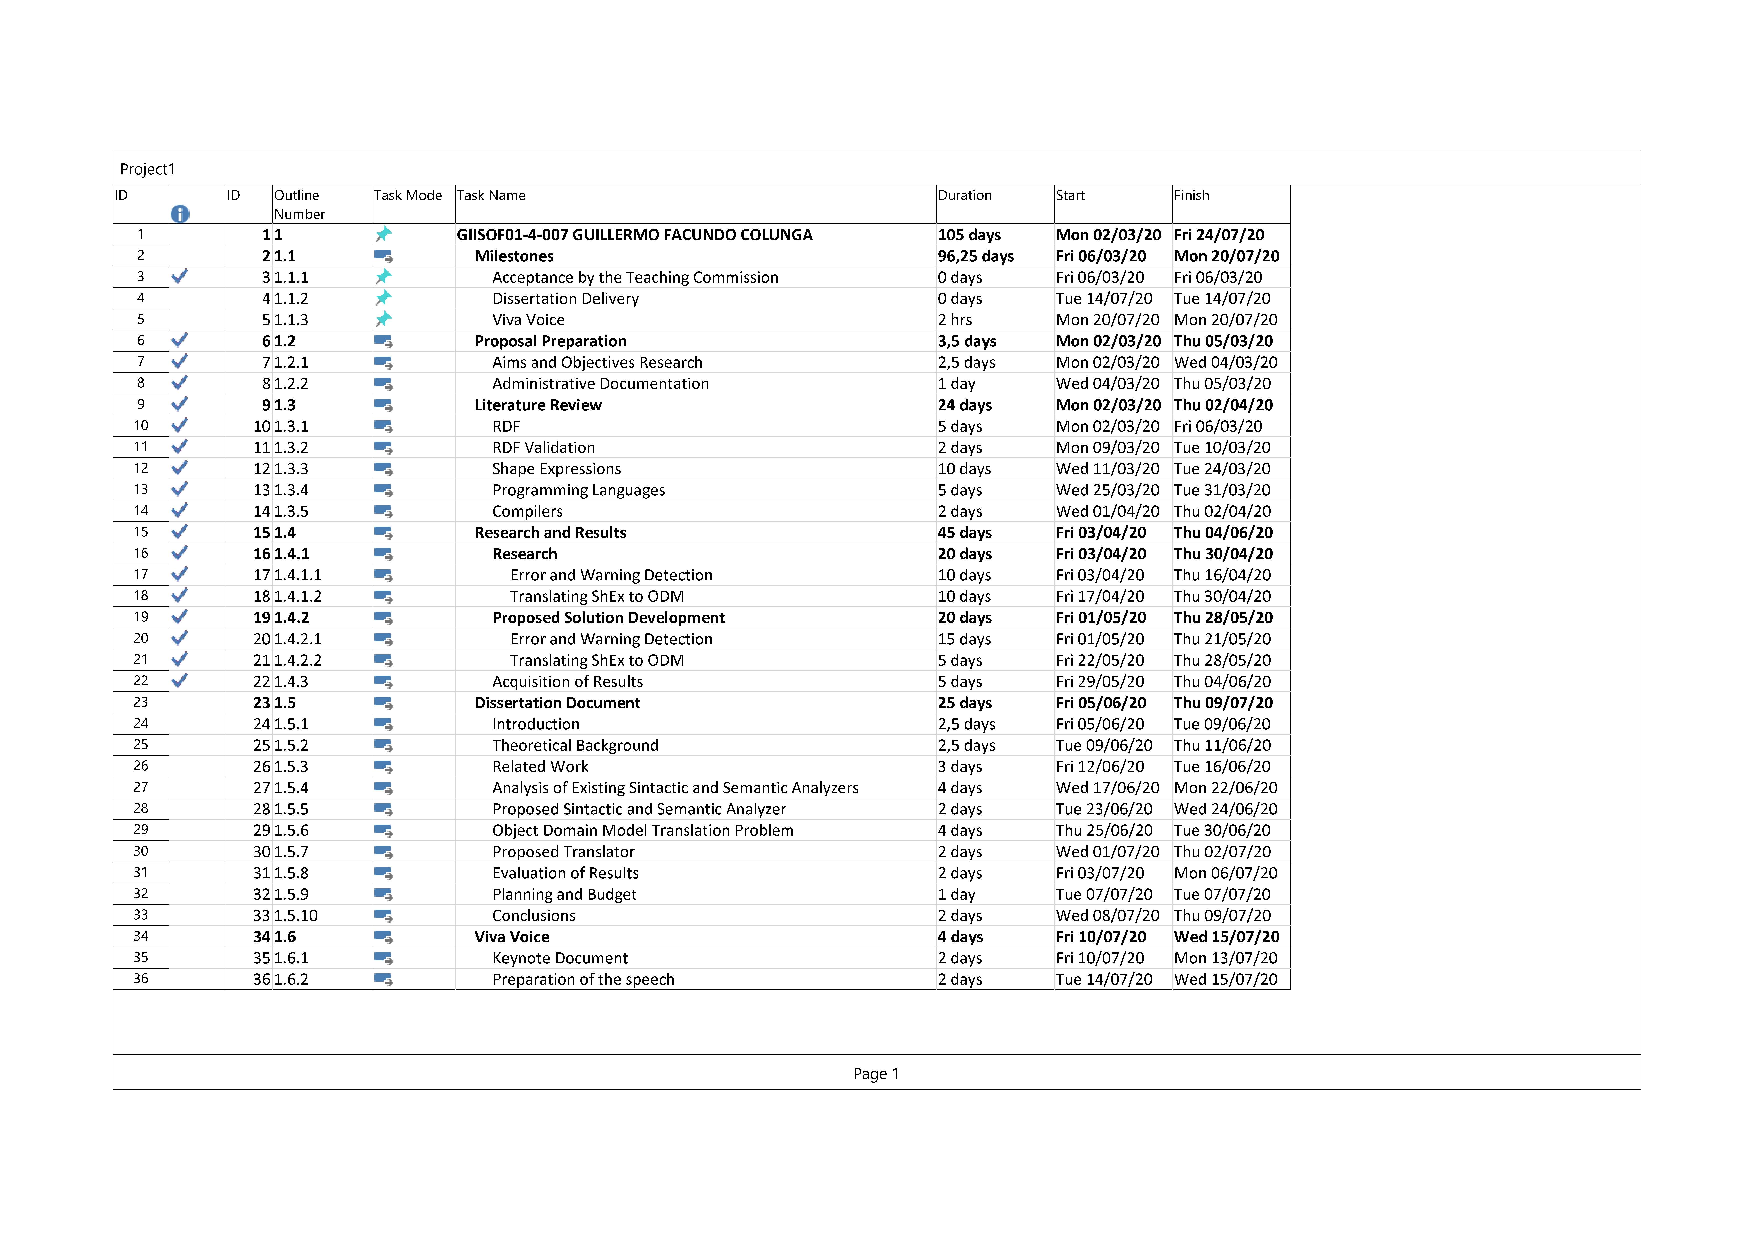
\includegraphics[width=\textwidth]{images/planificacion.pdf}
    \centering
	\caption[Tasks planning of the project]{Tasks planning of the project.}
    \label{fig:planning-sheet}
\end{figure}

\section{Budget}
To calculate this project we will take into account the estimate. From the estimation we can obtain
the time that is dedicated to each of the phases, in addition we have to take into account that not
all tasks are performed by the same profile and therefore not all profiles will have the same remuneration.
In our case as we separated the work in three phases we will also decompose the budget in three phases. The
\textbf{Proposal Preparation}, the \textbf{Research} and the \textbf{Development}.

In order to take the hourly wage we use the \url{https://www.salary.com} which aims to offer reliable
information about hourly wages per role.

\subsection{Proposal Preparation}
The proposal preparation computes all the administrative works and the previous researchs. This phase is performed
by a researcher profile.

\begin{figure}[h!]
    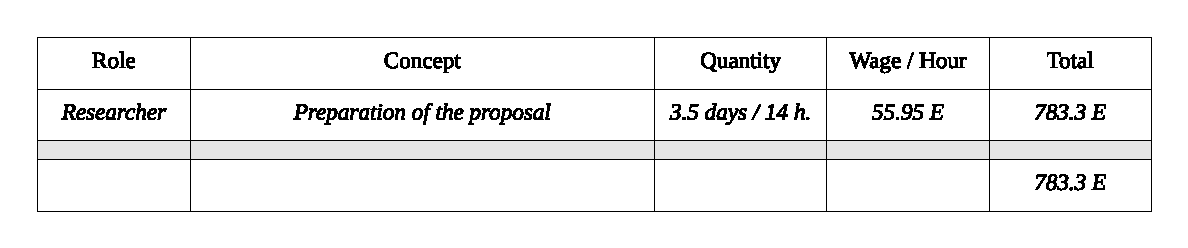
\includegraphics[width=\textwidth]{images/budget-proposal.pdf}
    \centering
	\caption[Proposal preparation costs]{Proposal preparation costs.}
    \label{fig:budget-proposal}
\end{figure}

\subsection{Research}
The research phase computes research works, including the analisys performed and the writing of the dissertation.
This phase is performed by a researcher profile.

\begin{figure}[h!]
    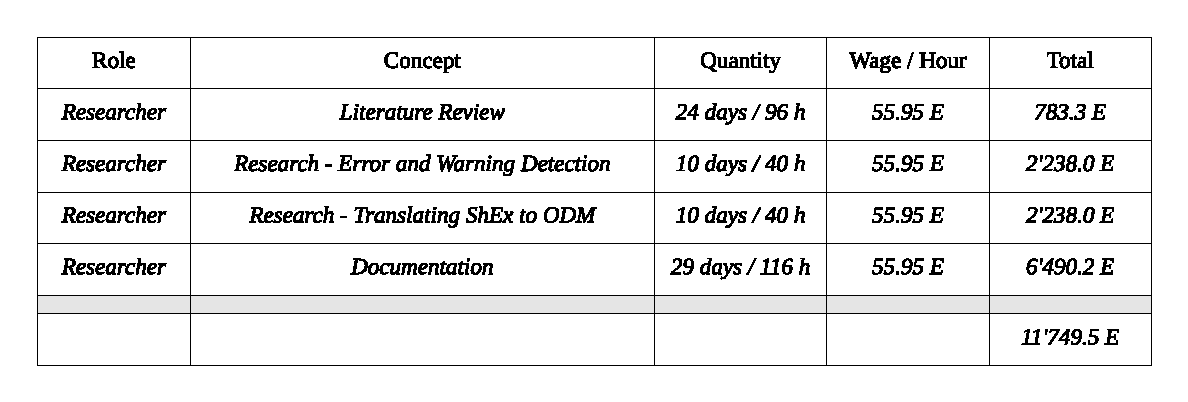
\includegraphics[width=\textwidth]{images/budget-research.pdf}
    \centering
	\caption[Research costs]{Research costs.}
    \label{fig:budget-research}
\end{figure}

\subsection{Development}
The development tasks are done to create a Probe Of Conocept (POC) that validates the proposed solution. This taska are not carried out by a researcher
but by an Scala Software Developer.

\begin{figure}[h!]
    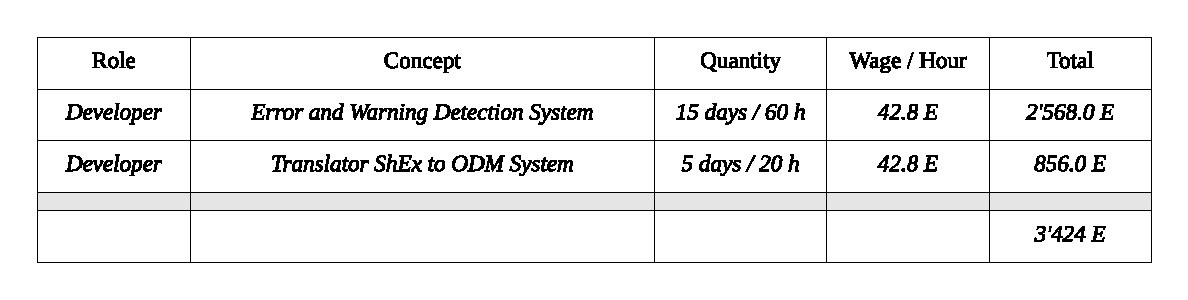
\includegraphics[width=\textwidth]{images/budget-development.pdf}
    \centering
	\caption[Development costs]{Development costs.}
    \label{fig:budget-development}
\end{figure}

\subsection{Aggregated Costs}
After calculating the partial costs of each of the phases of the project, the costs are added,
obtaining the value of the real cost of executing the project. To this is added a 10% that comes
from adding all the indirect costs of the project and the corresponding taxes. With all this we
obtain the final cost of our project. It is important to remember that being a research project,
the benefits are the project itself and this is a cost estimate.

\begin{figure}[h!]
    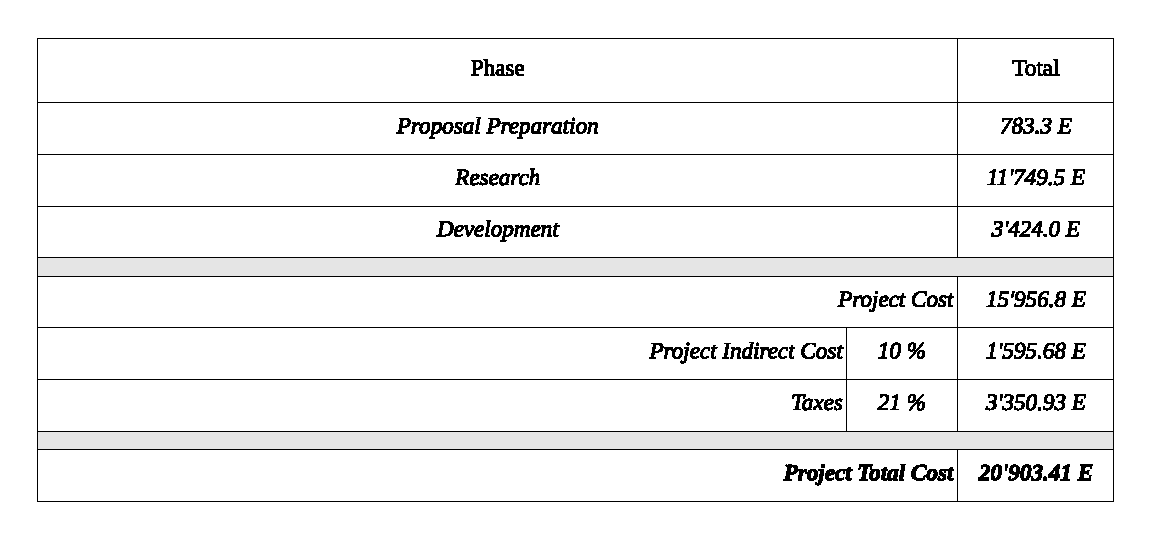
\includegraphics[width=\textwidth]{images/budget-general.pdf}
    \centering
	\caption[Aggregated costs]{Aggregated costs.}
    \label{fig:budget-general}
\end{figure}